% % % % % % % % % % % % % % % % % % % % % % % % % % % %
% Vorlage für ein Poster 
% Versionshistorie
% v1 erstellt von Dr. Thorsten Strempel
% v2 überarbeitet von Thorsten Bücking
% v2.1 Qullenangeben wie in der Vorlage zur Bachelorarbeit abgeändert
%      Umstellung der Literaturangaben auf BibLaTeX (Am besten mit biber verwenden, siehe Optionen im TeXstudio)
%v3 angepasst von Prof. Dr. Melanie Siegel
% % % % % % % % % % % % % % % % % % % % % % % % % % % %

%!!!!!!!!!!!!!!!!!!!!!!!!!!!!!!!!!!!!!!!!!!!!!!!!!!!!!!!!!!!!!!!!!!
% Die Datei "beamerthemeconfposter.sty" ist erforderlich, 
%         da hier einige Einstellungen vorgenommen wurden
%!!!!!!!!!!!!!!!!!!!!!!!!!!!!!!!!!!!!!!!!!!!!!!!!!!!!!!!!!!!!!!!!!!



\documentclass[final]{beamer}
%\documentclass[draft]{beamer}

\usepackage[english,german]{babel}

\usepackage[utf8]{inputenc}

% Stellt nützliche Befehle zum Erstellen von Postern bereit.
\usepackage[scale=1]{beamerposter} % Use the beamerposter package for laying out the poster

\boldmath

\usetheme{confposter} % Use the confposter theme supplied with this template

\setbeamercolor{block title}{fg=ngreen,bg=white} % Colors of the block titles
\setbeamercolor{block body}{fg=black,bg=white} % Colors of the body of blocks
\setbeamercolor{block alerted title}{fg=white,bg=dblue!70} % Colors of the highlighted block titles
\setbeamercolor{block alerted body}{fg=black,bg=dblue!10} % Colors of the body of highlighted blocks
% In der Datei "beamerthemeconfposter.sty" sind noch viele andere Farben zu finden.


%Durch passendes Auskommentieren kann gewählt werden, ob das Poster in Hoch- oder Querformat dargestellt werden soll

%Querformat
%\setlength{\paperwidth}{48in} % A0 landscape: width=46.8in, height=33.1in
%\setlength{\paperheight}{36in} 

%Hochformat, einmal in Inch und einmal im mm
%\setlength{\paperwidth}{36in} % A0 Portrait: width=33.1, height=46.8in
%\setlength{\paperheight}{48in} 
%oder
\setlength{\paperwidth}{841mm}
\setlength{\paperheight}{1189mm} 


%http://tex.stackexchange.com/questions/91572/changing-font-size-of-list-items-and-subitems
\setbeamertemplate{itemize/enumerate body begin}{\normalsize}
\setbeamertemplate{itemize/enumerate subbody begin}{\normalsize}
\setbeamertemplate{itemize/enumerate subsubbody begin}{\normalsize}

%-----------------------------------------------------------

\usepackage{graphicx}  % Zum Einbinden von Bildern
\usepackage{booktabs} % Top and bottom rules for tables
\usepackage{geometry}
\usepackage{listings} % Zum Darstellen von Quellcode

\lstdefinestyle{tksMathematica}{
	language=Mathematica,
	tabsize=2,
	basicstyle=\ttfamily\small,%       generell Schreibmaschinenschrift
	commentstyle=\color{blue},%  Kommentar blau
	keywordstyle=\color{red},%   Schlüsselwörter rot
	stringstyle=\color{DarkGreen},
	stringstyle=\ttfamily, % typewriter type for strings
	numbers=left,%               links Zeilennummern
	stepnumber=1,
	numberstyle=\scriptsize\ttfamily,
	numbersep=2em,
	backgroundcolor=\color{Gray},
	frame=lines,
	captionpos=b}

%----------------------------------------------------------------------------------------
%	Titel des Posters
%----------------------------------------------------------------------------------------

\title[Poster]{Bridging the Syn-to-Real Gap in Microorganism Detection Using Blended Synthetic Data} % Postertitel
\author[NN]{
Sebastian Jörz\textsuperscript{1},
Stefan Höreth\textsuperscript{2},
Antonio Jorba\textsuperscript{3},
Eva Brucherseifer\textsuperscript{1}
}
\institute[short]{%
\textsuperscript{1} Darmstadt University of Applied Sciences, Germany\\
\textsuperscript{2} Entega Abwasserreinigung GmbH \& Co. KG, Germany\\
\textsuperscript{3} COUNT+CARE GmbH \& Co. KG, Germany
}
\date{08.07.2025 v1}

\def\tbibitem#1#2#3#4{\bibitem{#1} \textbf{#2}, \textsc{#3}, #4}

\usepackage{amsmath,amsthm, amssymb, latexsym}

%----------------------------------------------------------------------------------------

\addtobeamertemplate{block end}{}{\vspace*{2ex}} % White space under blocks
\addtobeamertemplate{block alerted end}{}{\vspace*{2ex}} % White space under highlighted (alert) blocks
%\addtobeamertemplate{block begin}{}{\setlength{\parskip}{\baselineskip}} % 35pt plus 1pt minus 1pt}}

\setlength{\belowcaptionskip}{2ex} % White space under figures
\setlength\belowdisplayshortskip{2ex} % White space under equations
%\renewcommand{\baselinestretch}{1.5}

\newenvironment<>{definitionblock}[1]{%
  \setbeamercolor{block title}{fg=white,bg=red!75!black}%
  \begin{block}#2{#1}}{\end{block}}
\newenvironment<>{remarkblock}[1]{%
  \setbeamercolor{block title}{fg=white,bg=blue!75!black}%
  \begin{block}#2{#1}}{\end{block}}


% Literaturverzeichnis
\usepackage[backend=biber, style=numeric-comp, maxcitenames=2, doi=true, url=false, isbn=false, natbib=true]{biblatex}



\addbibresource{lit.bib} 			% Einbinden der bib-Datei



	\begin{document}

% The entire poster is contained within a frame, and individual sections are separated by blocks
% [t] Content is displayed at the Top.
\begin{frame}[t,fragile]

% Environment for displaying columns, option [t] stands for Top in the display
\begin{columns}[t,totalwidth=0.95\paperwidth]

% The number of columns ("column") reflects the number of columns on the poster.

% An empty column can be used to create spacing between columns, e.g.
\begin{column}{0.025\paperwidth}\end{column}


% Start of the first column
\begin{column}{0.5\paperwidth}

% Change the colors and backgrounds of the block titles
\setbeamercolor{block title}{fg=red,bg=white}

\begin{alertblock}{Monitoring Microorganisms}

%Microbes as Sewage Plant Quality Indicators


% \begin{}

The number of different types of microorganisms is an indicator for the quality of the sewage plant process. 
% This process should be automated using YOLO object detection.

\hfill\parbox[t]{0.5\linewidth}{
\begin{itemize}
    
\item \textbf{Overarching Goal:}
\begin{itemize}
\item Activated Sludge Monitoring
\item Automated using YOLO object detection

 % \item \textbf{Number of real Data:} x
 % \item \textbf{Idea:} Generate Synthetic Images

\end{itemize}
\end{itemize}
}\parbox[t]{0.5\linewidth}{
\begin{itemize}

 \item \textbf{Challenge:}
	\begin{itemize}
		\item Limited Data
            \item Homogeneous Data
	\end{itemize}

\end{itemize}
}\hfill

\end{alertblock}

%\medskip
\vspace*{-5mm}

% Change the colors and backgrounds of the block titles
\setbeamercolor{block title}{fg=ngreen,bg=white}


% Dataset, Source, Statistics (Number of entries, Labels, Class distribution)
\begin{block}{The \textbf{Domain Gap:} Muddy vs. Clear}
% The \textbf{Domain Gap:} Muddy vs. Clear
\begin{itemize}
    \item \textbf{Idea:} Expand dataset with public data
    \item \textbf{Challenge:} Different domains
    \item \textbf{Generalisation:} Models struggle with real-world sewage data (our dataset) vs. clean public datasets~\cite{rangel_dacosta_robust_2024}
    % \begin{itemize}
    %     \item 
    % \end{itemize}
    % \item \textbf{Domain Gap:} Public datasets are different from our dataset, as our dataset is captured with other microscopes and other surroundings around the microorganism.
    
        \begin{center}
        \begin{minipage}{0.45\linewidth}
            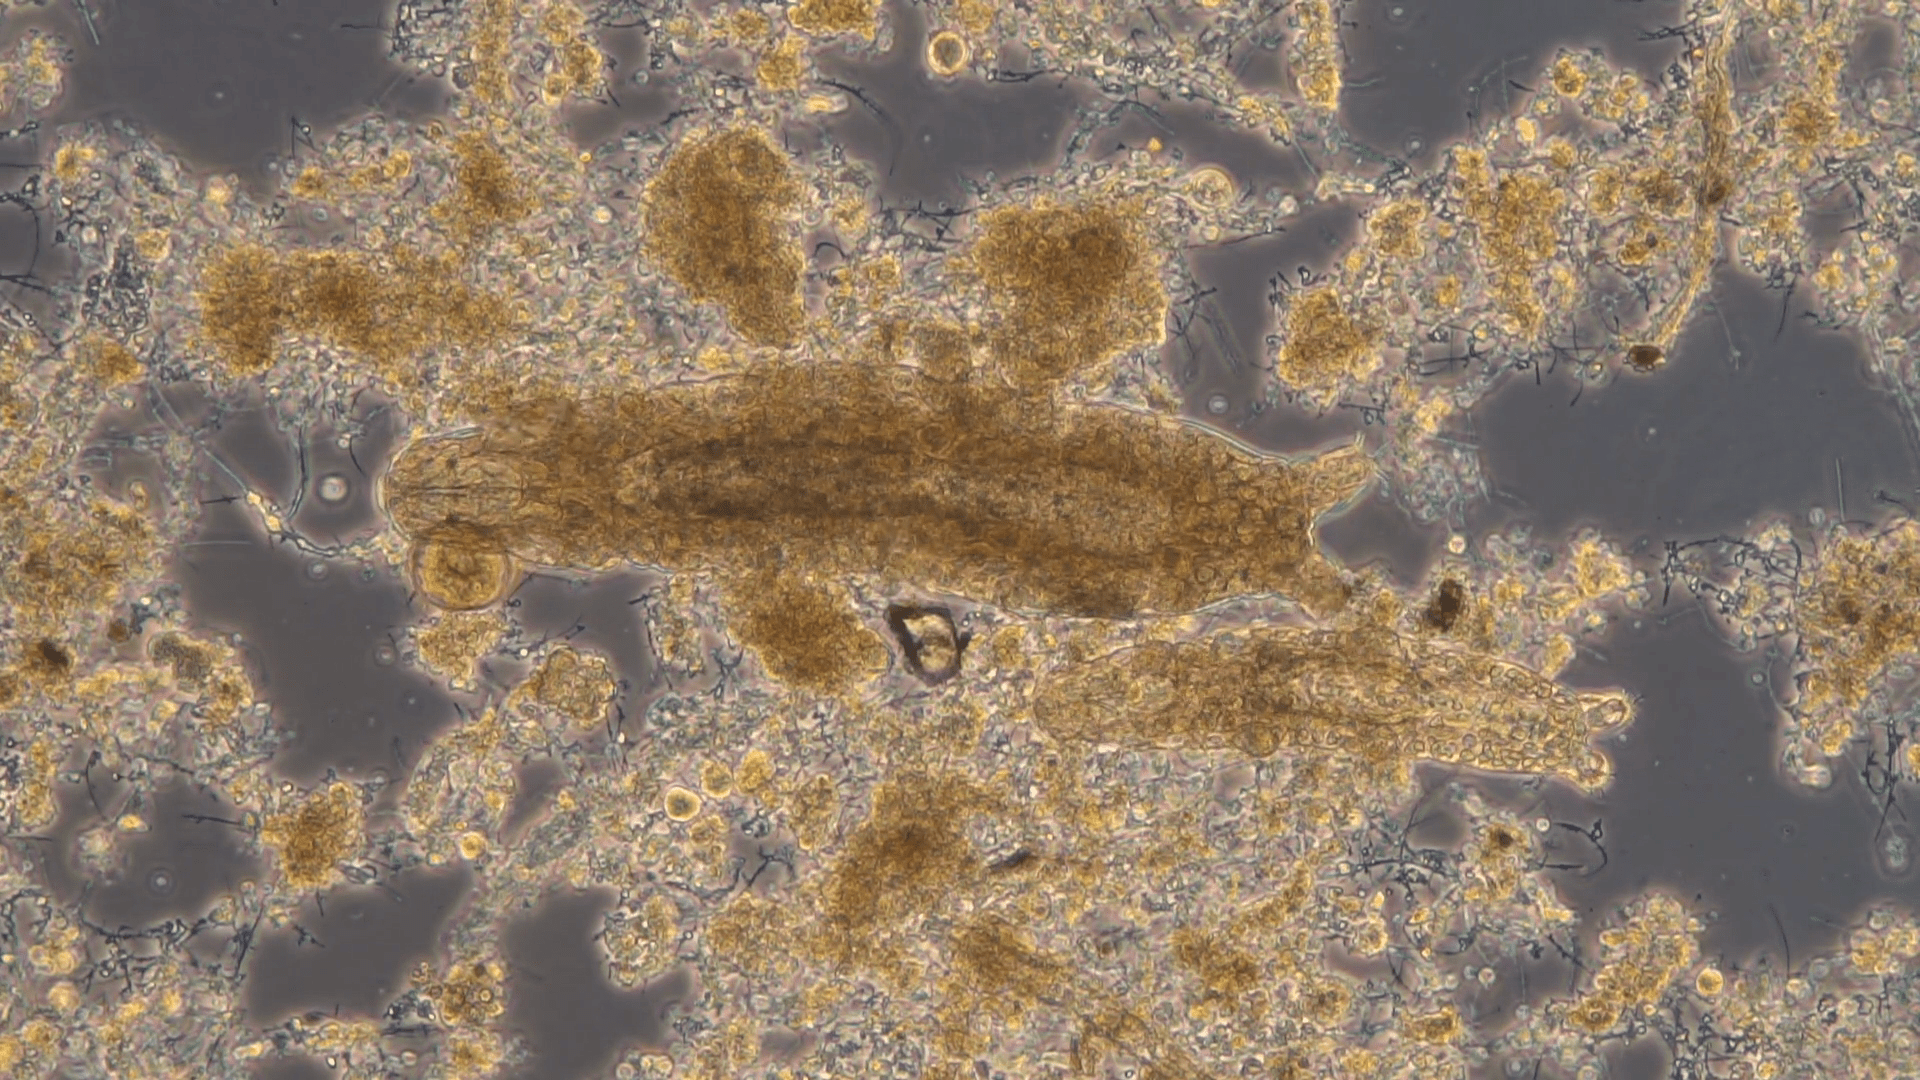
\includegraphics[width=\linewidth]{assets/Tardigrade_01_0003-min.png}
            \centering
            \small Tardigrades in a muddy environment (e.g. in
sewage plants). Source: own image
        \end{minipage}
        \hfill
        \begin{minipage}{0.45\linewidth}
            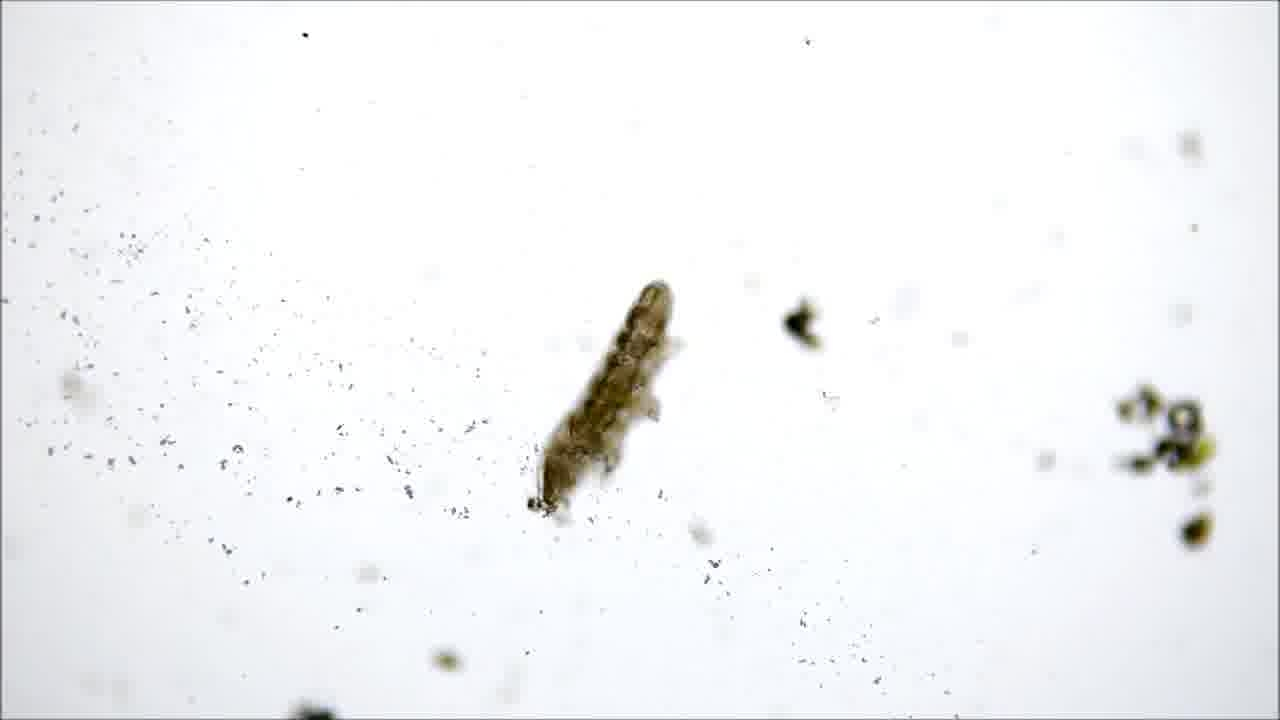
\includegraphics[width=\linewidth]{assets/Tardigrade_0429-2.jpeg}
            \centering
            \small Tardigrade in a clear environment. Source: \protect\parencite{jaso_tardigrade_2022}
        \end{minipage}
        \end{center}
\end{itemize}
\end{block}



\begin{block}{Our \textbf{Solution:} Synthetic Data Augmentation}
% Our \textbf{Solution:} Synthetic Data Augmentation
\begin{itemize}
    \item Generate synthetic data for our \textbf{'muddy' domain}
    \item Method: \textbf{Cut-Paste} (overlaying objects on varied backgrounds)
    \item Challenge: \textbf{Syn-to-Real Gap} (unrealistic composites, pixel artifacts)
\end{itemize}
    \begin{figure}[htbp]
        \centering
        \includegraphics[width=0.95\linewidth]{assets/pipeline-with-real.drawio.png}
        \caption{Procedure of the pipeline. Adapted from:~\parencite{dirr_cut-paste_2024}}
    \end{figure}	
\end{block}


\begin{block}{Reduce the Syn-to-Real Gap}
	% Tf-IDF with 3 PCA Components and then Image
    % Bridging the Gap: \textbf{Blending Techniques}
    \begin{itemize}
        \item \textbf{Blending:} Integrates objects seamlessly
        \item \textbf{Methods:} 
        \begin{itemize}
            \item \textbf{Alpha} blending
            \item \textbf{Gaussian} blending
            \item \textbf{Poisson} blending
            \item \textbf{Pyramid} blending
            \item \textbf{Multi-Blending} (Combination)
        \end{itemize}
    \item Example of an Alpha Mask blended with Gaussian blending:
\begin{center}
        \begin{minipage}{0.48\linewidth}
            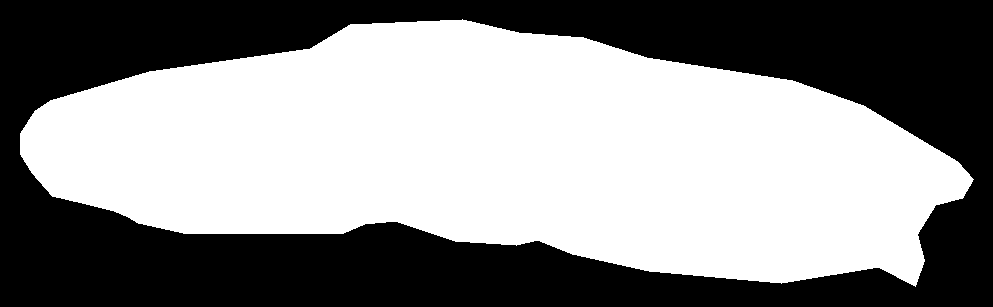
\includegraphics[width=\linewidth]{assets/mask.png}
            \centering
            \small Alpha Mask
        \end{minipage}
        \hfill
        \begin{minipage}{0.48\linewidth}
            
\includegraphics[width=\linewidth]{assets/blurred_mask.png}
            \centering
            \small Blurred Alpha Mask with Gaussian blending
        \end{minipage}
        \end{center}
        
    \end{itemize}
\end{block}

\begin{block}{Evaluation \& Datasets}
% \textbf{Experimental Design}
\begin{itemize}
    \item \textbf{Real Data:} Our In-Domain (\textbf{muddy}) \& Public Cross-Domain (\textbf{clear}) datasets
    \item \textbf{Datasets for Evaluation:}
    \begin{itemize}
        \item \textbf{T1: Baseline} (Real Data Only)
        \item \textbf{T2: Single Blending} (Alpha, Gaussian, Poisson, Pyramid)
        \item \textbf{T3: Multi-Blending} (Alpha + Gaussian + Pyramid)
    \end{itemize}
    \item Varying \textbf{Synthetic Ratios}: 0\%, 30\%, 60\%, 90\%, 100\%
    % \item \textbf{T1 (Baseline):} In-Domain + Cross-Domain real images
    % \item \textbf{T2 (Single Blending Method):} In-Domain + Cross-Domain + Synthetic (In-Domain objects on In-Domain backgrounds) using Alpha, Gaussian, Poisson, or Pyramid blending individually.
    % \item \textbf{T3 (Multiple Blending Methods):} In-Domain + Cross-Domain + Synthetic (In-Domain objects on In-Domain backgrounds) using a combination of Alpha, Gaussian, and Pyramid blending.
    % \item \textbf{Ratios:} 0\%, 30\%, 60\%, 90\%, 100\% synthetic data
    \item \textbf{Test Set:} 223 In-Domain images
    \item \textbf{Model:} YOLOv11m (25 Epochs)
    \item \textbf{Evaluation Metrics:}
    \begin{itemize}
        \item mAP@[0.50:0.95] (Object detection performance)
        \item FID \& CMMD (Image Quality / Syn-Real Gap)
    \end{itemize}
%     \item Eval: MAP
% \item \textbf{Quantify:} 
%         \begin{itemize}
%             \item Train a Yolo Model with different synthetic data
%             \item Measure using FID and CMMD (Embedded Space): Image Quality Metrics
%         \end{itemize}
\end{itemize}
%     \begin{table}[htbp]
%   \caption{Composition of training sets per input dataset. All sets with synthetic data total to 3413 images due to undersampling. The ratio (\%) refers to the portion of synthetic images in the final dataset.}
%   \centering
%   \setlength{\tabcolsep}{6pt}
%   \renewcommand{\arraystretch}{1.2}
%   \begin{tabular}{@{}l|rrrrr@{}}
%     \multicolumn{1}{c|}{} & \multicolumn{5}{c}{\textbf{Synthetic Data Ratio}} \\
%     \cmidrule(lr){2-6}
%     \textbf{Input Dataset} & \textbf{0\%} & \textbf{30\%} & \textbf{60\%} & \textbf{90\%} & \textbf{100\%} \\
%     \midrule
%     Cross-domain           & 3356 & 2349 & 1342 & 336  & \textemdash \\
%     In-domain              & 57   & 57   & 57   & 57   & \textemdash \\
%     Synthetic              & \textemdash & 1007 & 2014 & 3020 & 3356 \\
%     \midrule
%     \textbf{Total}         & \textbf{3413} & \textbf{3413} & \textbf{3413} & \textbf{3413} & \textbf{3413} \\
%     \bottomrule
%   \end{tabular}
%   \label{tab:trainset:split}
% \end{table}

\end{block}




%%%%%%%%%%%%%%%%%%%%%%%%%%%%%%%%%%%%%%%%%%%%%%%%%%%%%%%%%%%%%%%

% End of the first column
\end{column}


% An empty column for spacing between filled columns serves for a nicer display
\begin{column}{0.025\paperwidth}\end{column}


% Start of the second column
\begin{column}{0.4\paperwidth}



\begin{block}{Improved Detection: Before vs. After}
    \begin{center}
    \begin{minipage}{0.48\linewidth}
        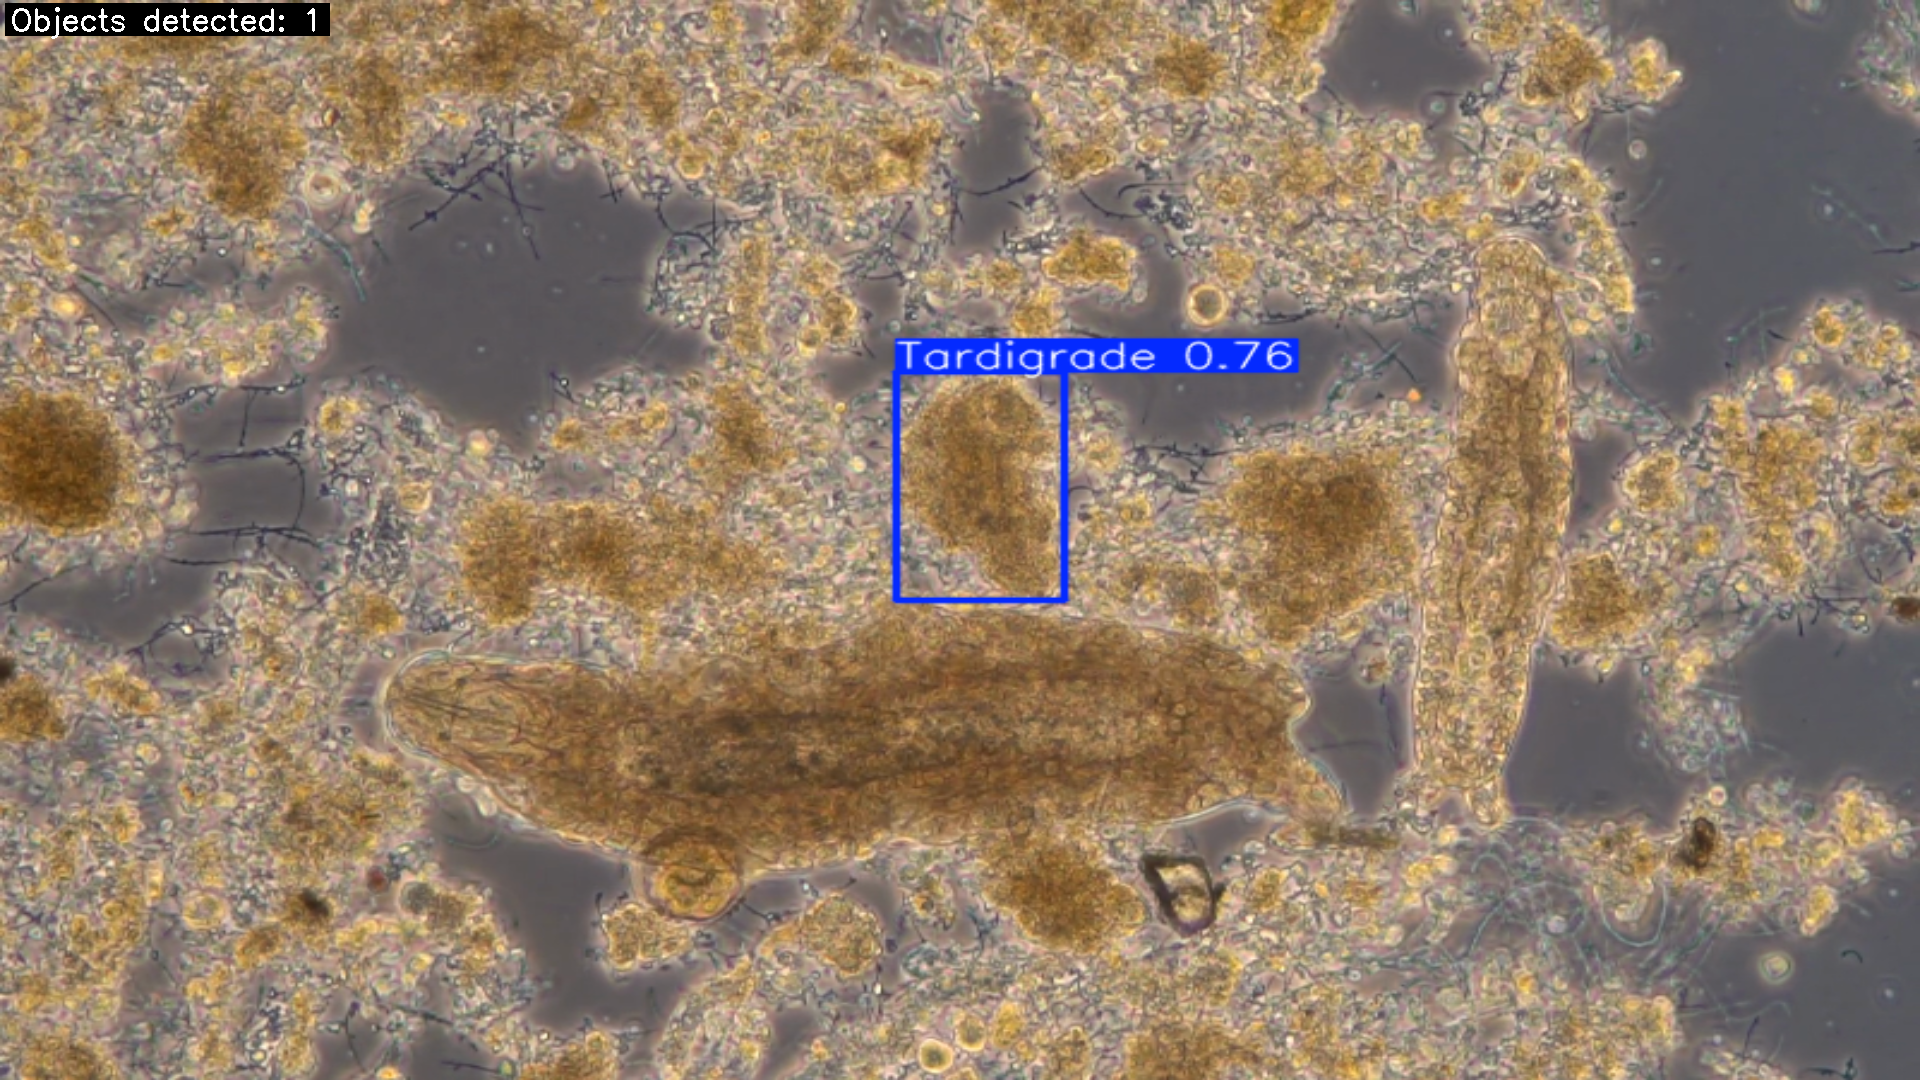
\includegraphics[width=\linewidth]{assets/best-t1.pt_Tardigrade_01_0028.png}
        \centering
        \small Prediction with a model trained on the T1 dataset (\textbf{Before})
    \end{minipage}
    \hfill
    \begin{minipage}{0.48\linewidth}
        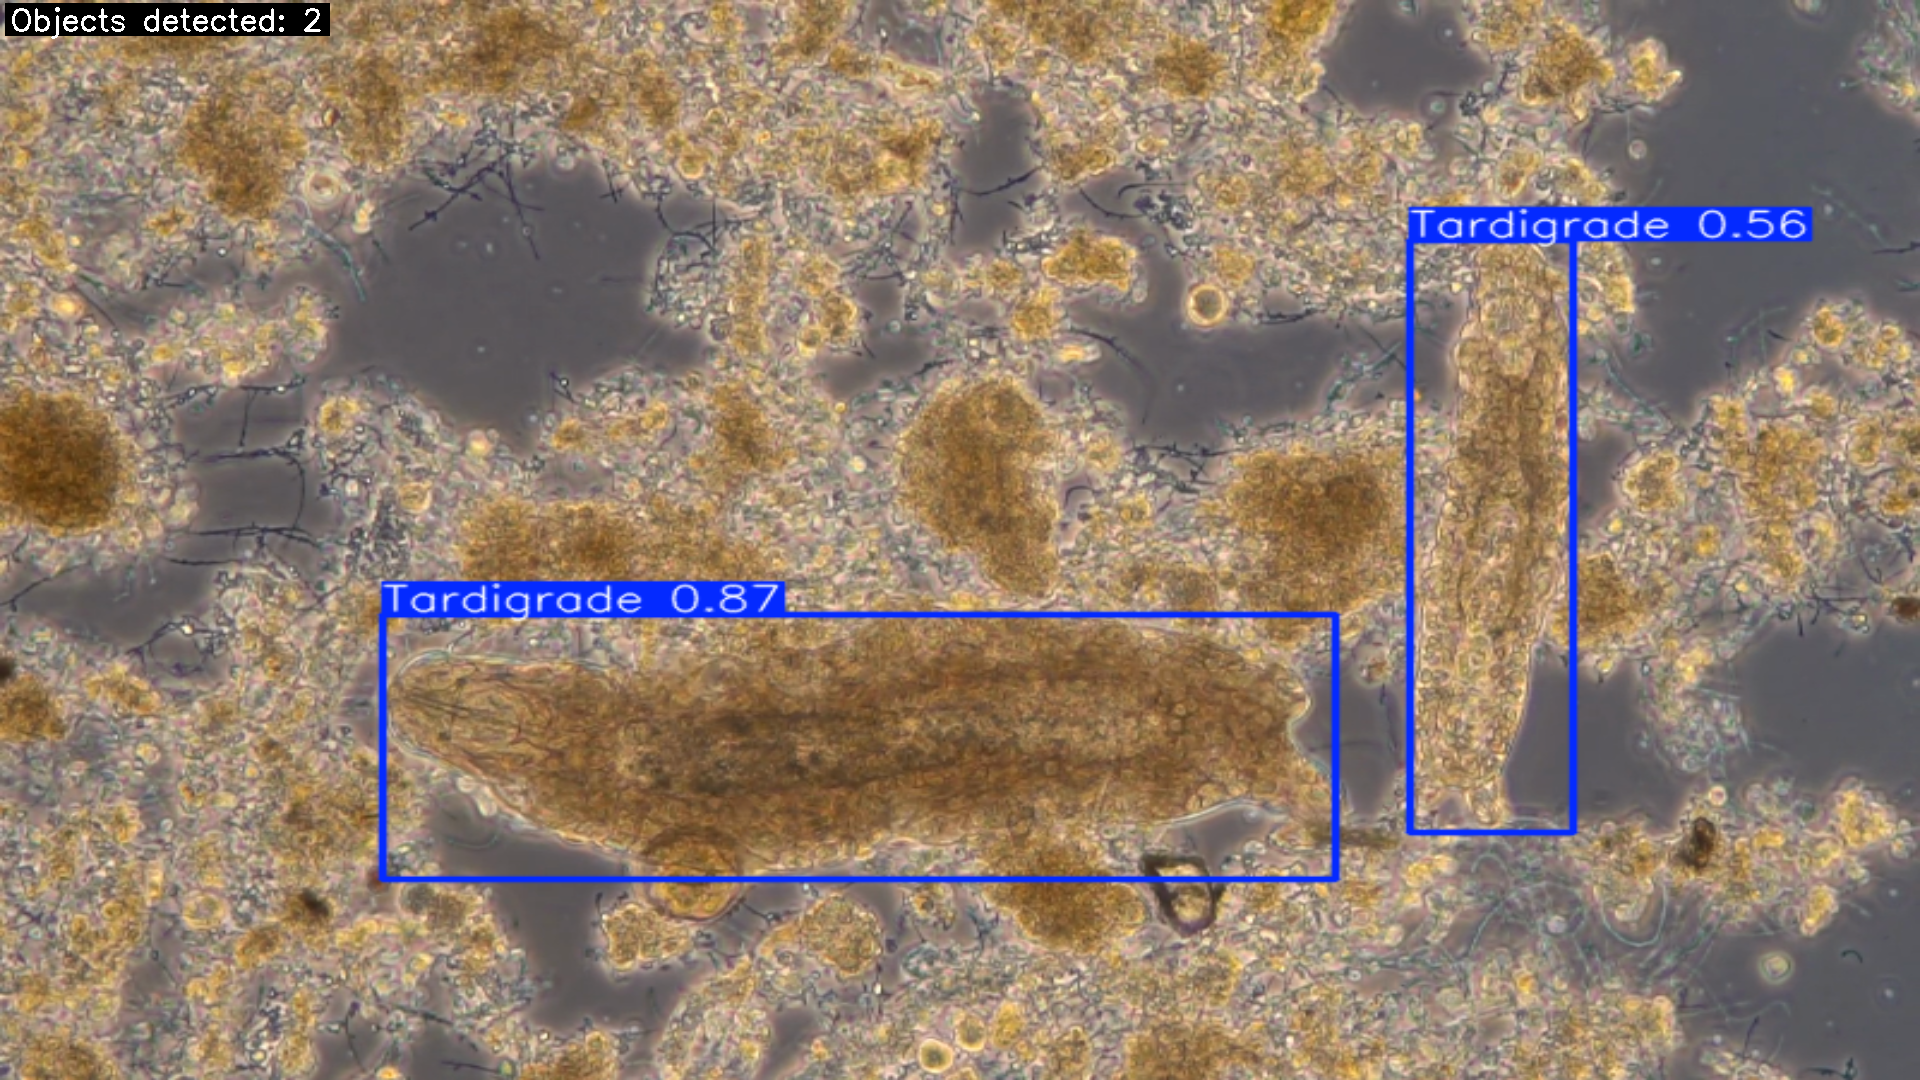
\includegraphics[width=\linewidth]{assets/best-t4.pt_Tardigrade_01_0028.png}
        \centering
        \small Prediction with a model trained on the T4 dataset (\textbf{After})
    \end{minipage}
    \end{center}
\end{block}



\begin{block}{Results}
\begin{itemize}
\item \textbf{mAP Performance (YOLOv11m):}


    % \item \textbf{Heatmap} for the self-trained model, trained with different types of blending methods and multiple ratios between real and synthic data.
    \begin{itemize}
        \item Baseline (T1): \textbf{0.58 mAP}
        \item Single Blending (T2): Up to \textbf{0.82 mAP} (Pyramid)
        \item Poisson Blending: Underperformed significantly (0.27 mAP)
        \item Multi-Blending (T3): \textbf{Best at 0.85 mAP}
        \item \textbf{Optimal Ratio:} 60\% Synthetic Data
    \end{itemize}
    \begin{figure}[htbp]
        \centering
        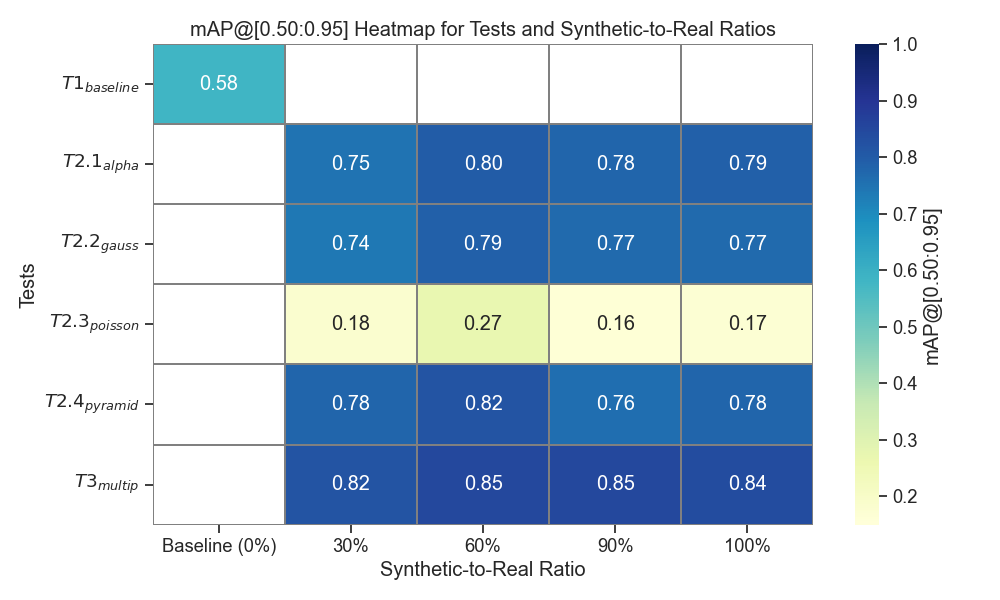
\includegraphics[width=0.95\linewidth]{assets/heat_plot_YlGnBu_map05-95.png}
        \caption{Heatmap of different models trained with different syn-to-real ratios and different blending methods}
    \end{figure}	

    \item \textbf{Image Quality (FID \& CMMD):}
    \begin{itemize}
        \item Lower scores = more realistic images
        \item T1 (Baseline): Highest scores (least realistic).
        \item \textbf{T3 (Multi-Blending): Lowest scores (most realistic)}
        \item Correlates with mAP (smaller gap = better detection).
    \end{itemize}
    \begin{figure}[htbp]
        \centering
        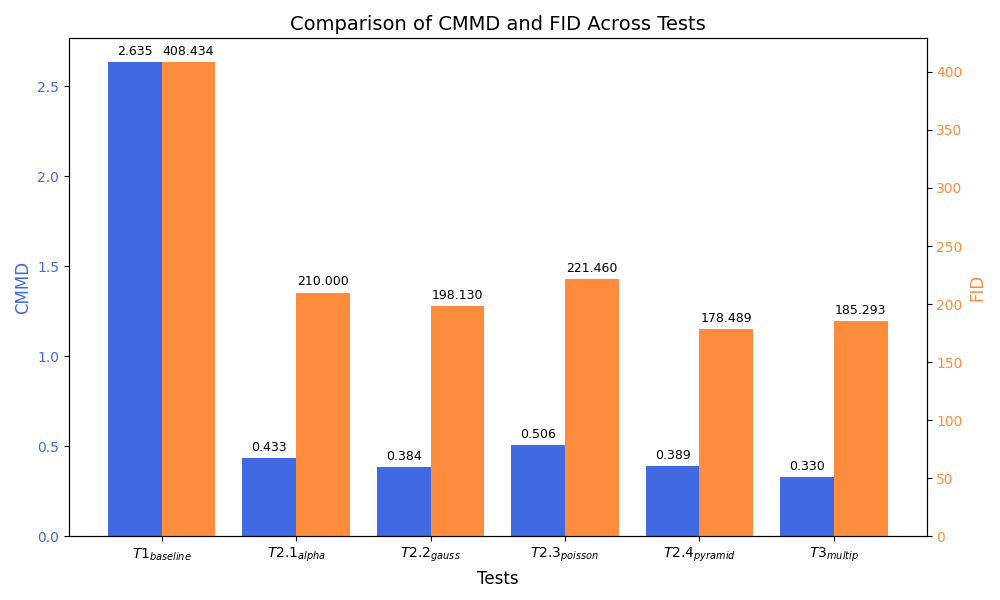
\includegraphics[width=0.95\linewidth]{assets/fid_cmmd_plot_transparent.png}
        \caption{FID and CMMD, calculated on different test datasets in relation to the real dataset of the muddy environment}
    \end{figure}	
\end{itemize}
  
\end{block}








\begin{block}{Conclusion \& Future Directions}
    \begin{itemize}
        \item \textbf{Synthetic data significantly boosts object detection in data-scarce domains}

\item \textbf{Blending methods are crucial} for reducing the syn-real gap
\item \textbf{Multi-blending excels}, yielding realistic images \& highest mAP

\item \textbf{Future Work:} Incorporate distractors (e.g., mud), noise, and explore more blending methods to enhance model resilience

    \end{itemize}
\end{block}




\vspace*{-10mm}

\begin{block}{References}

\printbibliography

\end{block}


% End of the second column
\end{column}

\end{columns}

\end{frame}

\end{document}
